\question (武汉理工大学,2005年)如果有多个中断同时发生,系统将响应中断优先级最高的中断请求。若调整中断时间的响应次序,可以采用
\par\twoch{中断禁止}{中断嵌套}{中断响应}{\textcolor{red}{中断屏蔽}}
\begin{solution}为了更灵活地运用中断,计算机中采用中断屏蔽技术。屏蔽的基本意思是让某种中断不起作用。确切地说,对每一个外部硬件中断源设置一个中断屏蔽位,约定该位为0为开屏蔽状态,为l表示处于屏蔽状态,当然也可以反过来约定。一个中断源在对应的中断屏蔽位为屏蔽状态的情况下,它的中断请求不能得到CPU的响应,或者干脆就不能向CPU提出中断请求。
\end{solution}
\question ( )不是常用三级时序系统中的一级
\par\twoch{\textcolor{red}{指令周期}}{机器周期}{节拍}{定时脉冲}
\begin{solution}A。 三级时序系统包括机器周期、节拍和工作脉冲。
归纳总结:三级时序系统是小型机常用的时序系统,在机器周期间、节拍电位间、工作脉冲间既不允许有重叠交叉,也不允许有空隙,应该是一个接一个的准确连接。
\end{solution}
\question 下列叙述中,正确的有
\par\fourch{计算机三级时序是指机器周期、指令周期和存储周期}{\textcolor{red}{CPU只有在执行PUSH和POP指令后,堆栈寄存器(SP)的值才能递加或递减}}{指令有时候根据PC,有时候根据转移指令从主存中读出}{全对}
\begin{solution}B。 A错误,因为计算机的三级时序是指CPU周期、节拍电位、节拍脉冲。 B正确。
C错误,程序计算器PC,用以指出下一条指令在主存中的存放地址。CPU正是根据PC的内容去主存取得指令的。转移指令也是通过改变PC的值,来达到程序控制的目的的。故指令总是根据程序计数器PC从主存中读出的。
D错误。 因此,本题应该选择B。
\end{solution}
\question 一般情况下,采用下列哪种编码方式时,微指令的控制字段位数最多
\par\twoch{\textcolor{red}{直接编码方式}}{字段直接编码方式}{字段间接编码方式}{以上都不对}
\begin{solution}A。
采用直接编码方式时,每个微操作命令都对应控制字段中的1位控制位,此时控制字段位数最多。
\end{solution}
\question 计算机执行乘法指令时,由于其操作复杂,需要更多的时间,通常采用(
)控制方式
\par\twoch{异步控制}{延长机器周期内的节拍数}{\textcolor{red}{中央控制与局部控制相结合}}{同步控制与异步控制相结合}
\begin{solution}C。 乘法指令属于中央控制与局部控制相结合的典型特例。
归纳总结:中央控制与局部控制相结合的方式可以将执行周期需要更多时钟周期的指令安排局部控制节拍,并将其插入到中央控制的执行周期内。
\end{solution}
\question 下列有关微指令格式的描述中,错误的是
\par\fourch{相对于直接编码(控制)方式,字段直接编码方式的控存利用率更高}{相对于字段直接编码方式,直接编码(控制)方式的执行速度更快}{相对于断定法(下指字段法),采用增量计数器法的微指令格式更短}{\textcolor{red}{相对于水平型微指令,一条垂直型指令中包含的微命令更多}}
\begin{solution}D。
直接编码方式不需要译码,但微指令字长过长。字段直接编码方式,缩短了微指令字长,但因为要通过译码电路再发出微命令,因此比直接编码方式慢。故A和B都是正确的描述。
采用断定法,需要多一个下地址字段,而增量计数器法不需要,故采用增量计数器法的微指令格式更短,故C正确。
水平型指令的特点是一次能定义并执行多个并行操作的微指令,而垂直型微指令通常只有1\textasciitilde{}2个微命令,不强调并行控制功能,故水平型微指令包含的微指令更多。
故D描述错误。
\end{solution}
\question 在控制器的控制方式中,机器周期内的时钟周期个数可以不相同,这属于
\par\twoch{\textcolor{red}{同步控制}}{异步控制}{半异步控制}{联合控制}
\begin{solution}A。
同步控制方式下机器周期内时钟周期个数可以相等或不相等,而异步控制方式没有统一的时钟控制,采用应答方式实现。这里强调机器周期,所以应为同步控制方式。
\end{solution}
\question 下列关于微指令编码方式的说法中,错误的是
Ⅰ.字段直接编码可以用较少的二进制信息表示较多的微操作命令信号,如有两组互斥微命令中,微命令个数分别为8和9,则只分别需要3位和4位即可表示
Ⅱ.直接编码无须进行译码,微指令的微命令字段中每一位都代表一个微命令
Ⅲ.垂直型微指令以较长的微程序结构换取较短的微指令结构,因而执行效率、灵活性都高于水平型微指令
Ⅳ.字段间接编码中,一个字段的译码输出需要依靠另外某一个字段的输入
\par\twoch{\textcolor{red}{Ⅰ、Ⅲ和Ⅳ}}{Ⅱ、Ⅲ和Ⅳ}{Ⅱ和Ⅳ}{Ⅰ、Ⅱ、Ⅲ和Ⅳ}
\begin{solution}A。
编码的是对微指令的控制字段进行编码,以形成控制信号;目的是在保证速度的情况下,尽量缩短微指令字长。
微命令个数为8时,需要4位,假设只用3位,将会造成每个编码都会输出一个微命令,事实上,微命令的编码需要预留一个字段表示不输出,Ⅰ错误。垂直型微指令的缺点是微程序长、执行速度慢、工作效率低,Ⅲ错误。字段间接编码中的一个字段的某些微命令还需由另一个字段中的某些微命令来解释,即受到某一个字段的译码输出,Ⅳ错误。
\end{solution}
\question 某机共有70个微控制信号(即微命令),构成6个互斥的微命令组,各组分别包含8、11、3、16、7、25个微命令。如果采用字段直接编码方式,微指令的控制字段需要(
)位
\par\twoch{21}{22}{\textcolor{red}{23}}{25}
\begin{solution}C。
采用字段直接编码方式时,每个字段除要发出微命令外,还需要能够表示不发出任何微命令的状态,故每个字段需要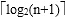
\includegraphics[width=0.68750in,height=0.19792in]{computerassets/192b018e4f8f9385b44d3c130841491a.jpeg}位,n为该字段包含的微命令组。
故微指令的操作控制字段所需位数为4+4+2+5+3+5=23,即控制字段需要23位。
知识点回忆:
如果本题用直接控制方式的话,其控制字段需要8+11+3+16+7+25=70位。相比于直接编码(直接控制方式),字段直接编码方式缩短了微指令的字长,但增加了译码的时间。
\end{solution}
\question 下表给出了5条微指令I1~I5所发出的控制信号a~j。设计微指令的控制字段,要求保持微指令本身的并行性,需要的最少的控制位数为
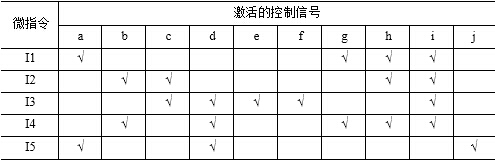
\includegraphics[width=3.33333in,height=1.08333in]{computerassets/5b1bab1abb87d9250f00d12856549ee7.jpeg}
\par\twoch{6}{\textcolor{red}{7}}{8}{10}
\begin{solution}B。 微指令的编码方式主要有以下几种: (1)直接编码(直接控制)方式
(2)字段直接编码方式 (3)字段间接编码方式 (4)混合编码(一般不考查)
前3种编码方式,后者都比前者进一步缩短微指令字长,即控制位数是递减的。但题目要求保持微指令本身的并行性,由于(3)中某些微命令还需由另一个字段中的某些微命令来解释,即其微指令并行能力受到削弱。故本题应该是采用字段直接编码方式。
分析如下:
1)将出现情况完全相同的控制信号合并。观察表格可发现,控制信号e、f只在微指令I3中同时出现,可合用1位控制位来表示。
2)分析微指令的兼容、互斥情况。尽量将互斥的控制信号分在一组,采用字段直接编码法进行控制。观察表格可发现控制信号(a、b、e)是互斥的,(c、g、j)也是互斥的,因此可将(a、b、e)、(c、g、j)分别放在两个组内,每组经译码器输出各给出的3个控制信号,其余的d、h、i一个信号一组。下图是微指令控制字段格式图,其中字段的0或00统一表示``无操作''。

~
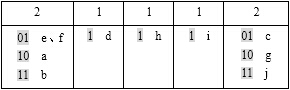
\includegraphics[width=3.02083in,height=0.93750in]{computerassets/4e16b737bedeef5f63b46047bbfe2996.jpeg}~

所以最少的控制位数为2+1+1+1+2=7。
\end{solution}
\question (西安交通大学,2003年)在控制单元的异步控制方式中,各种微操作的执行时间分配方案是
\par\fourch{所有微操作分配相同的执行时间}{\textcolor{red}{各个微操作需要多长时间就分配多长时间}}{大多数微操作分配较短的执行时间,某些复杂微操作分配较长的执行时间}{所有微操作在同一节拍中进行}
\begin{solution}B。
在异步控制方式中,每条指令需要多少节拍,就产生多少节拍;各个微操作需要多长时间就分配多长时间。异步控制方式不仅要区分不同指令对应的微操作序列的长短,而且要区分其中每个微操作的繁简,每个指令、每个微操作需要多少时间就占用多少时间,这种方式不再有统一的周期、节拍,各个操作之间采用应答方式衔接。
\end{solution}
\question (国防科技大学,2003年)在微程序控制中,执行指令微程序的首条微指令地址是通过(
)得到的
\par\twoch{程序计数器}{前条微指令}{uPC+1}{\textcolor{red}{指令操作码映射}}
\begin{solution}D。
在微程序控制中,执行指令微程序的首条微指令地址是通过指令操作码映射得到的,如下图所示:
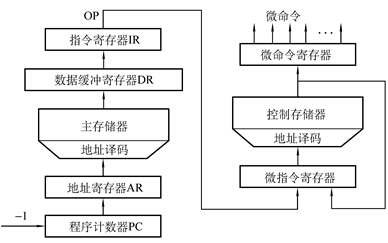
\includegraphics[width=4.04167in,height=2.53125in]{computerassets/da09d1d834c7788c8e364a45a793ee25.jpeg}
\end{solution}
\question (北京理工大学,2005年)为确定下一条微指令的地址,通常采用断定方式,其基本思想是
\par\fourch{用程序计数器(PC)来产生后继微指令地址}{用微程序计数器(uPC)来产生后继微指令地址}{\textcolor{red}{通过微指令顺序控制字段由设计者指定或由设计者指定的判别字段控制产生后继微指令地址}}{通过指令中指定一个专门字段来控制产生后继微指令地址}
\begin{solution}C。 断定方式是指后续微指令的地址可以由微指令的下地址字段直接给出。
\end{solution}
\question (上海交通大学,2000年)水平型指令与垂直型微指令相比
\par\twoch{前者一次只能完成一个操作}{\textcolor{red}{后者一次只能完成一个操作}}{两者都是一次只能完成一个操作}{两者都是一次完成多个操作}
\begin{solution}B。
水平型微指令具有良好的并行性,每条微指令可以完成较多的基本操作,但垂直型微指令接近于机器指令的格式,每条微指令只能完成一个基本微操作。
\end{solution}
\question (武汉大学,2002年)下列哪个选项不可能是微指令格式中的组成部分
\par\twoch{\textcolor{red}{操作码字段}}{操作控制字段}{外部条件字段}{下地址字段}
\begin{solution}A。 操作码字段属于机器指令的组成部分。
\end{solution}
\question (武汉大学,2002年)已知某CPU采用微程序控制方式,其控制存储器容量为512×32位。微程序可以在整个控制存储器中实现转移,控制微程序转移的条件有5个,微程序控制指令采用水平型格式,后继微地址采用断定方式,那么微指令中的3个字段:微命令、判别测试、下微地址分别为(
)位
\par\twoch{\textcolor{red}{18、5、9}}{9、5、9}{18、5、18}{9、5、18}
\begin{solution}A。
由于控制存储器容量为512×32位,可以得出控制存储器有512个存储单元,所以下微地址字段为9位(2\^{}9=512)。控制微程序转移的条件有5个,所以可以得知有5个判断条件。若采用直接表示法,则判别测试字段应为5位,每位表示一个测试条件。最终,可以得到微命令字段为(32-5-9)位=18位。
\end{solution}
\question 假设微操作控制信号用Cn表示,指令操作码译码器输出用Im表示,节拍电位信号用Mr表示,节拍脉冲信号用Ti表示,状态反馈信号用Bj表示,则硬布线控制器的基本原理可描述为
\par\twoch{Cn=f(Im,Ti)}{Cn=f(Im,Bj)}{Cn=f(Mr,Ti,Bj)}{\textcolor{red}{Cn=f(Im,Mr,Ti,Bj)}}
\begin{solution}D。
微操作控制信号=f(译码器输出,节拍电位信号,节拍脉冲信号,状态反馈信号)。
\end{solution}
\question (南京航空航天大学,2001年)微程序控制器与组合逻辑控制器相比主要优越之处是
\par\twoch{速度快}{\textcolor{red}{控制简单、规整}}{节省芯片面积}{用户编程方便}
\begin{solution}B。
微程序控制器同组合逻辑控制器相比,具有规整性、灵活性、可维护性等一系列优点。
\end{solution}
\question 下列选项中,( )不是发生中断请求的条件
\par\twoch{\textcolor{red}{一条指令执行结束}}{一次I/O操作结束}{机器内部发生故障}{一次DMA操作结束}
\begin{solution}A选项不是发生中断请求的条件,而是CPU响应中断的条件。
解题技巧:B选项是产生外部中断的条件;C选项是产生内部中断的条件;D选项是产生DMA结束中断的条件。采用排除法可以方便地得到结果。
\end{solution}
\question 设置中断屏蔽字可以动态地改变( )优先级
\par\twoch{中断查询}{中断响应}{\textcolor{red}{中断处理}}{中断返回}
\begin{solution}我们知道中断屏蔽是中断服务程序执行的,那么也就是说已经都经过了``中断响应''周期,也就不可能是改变中断响应的优先级,排除最可疑的选项B。而选项A和中断返回也都是明显的干扰项,本题正确答案选C。
\end{solution}
